\subsection{How Many Target Labels Are Needed?}
\label{sec:label-budget}

The single 50/50 target diagnostic answers whether adaptation can recover sensitivity, but not how much target annotation that recovery requires. We therefore fix the target test half and draw nested calibration subsets from the remaining target pool at 5\%, 10\%, 25\% and 50\% of all eligible target subjects. Each subset is drawn without replacement from the same shuffled pool, so the curve isolates calibration-set size rather than a change of test patients. The source threshold is evaluated on the same test half as the no-recalibration reference, and every recalibrated threshold is selected by the same patient-blocked procedure used elsewhere.


\begin{figure}[tb]
\centering
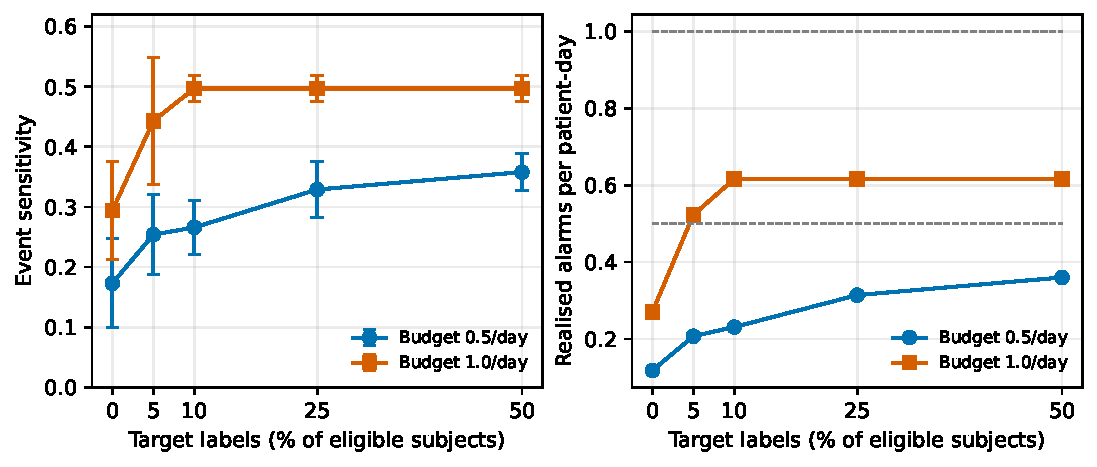
\includegraphics[width=\linewidth]{figures/label_budget.pdf}
\caption{Target label-budget curve for the logistic scorer, averaged over three source seeds. Left: event sensitivity versus the percentage of eligible target subjects used for threshold calibration; error bars are sample standard deviations over seeds. Right: realised alarms per patient-day against the requested budget (dashed lines), showing that label cost and operating point interact. The zero-label point applies the source threshold without target calibration.}
\label{fig:label-budget}
\end{figure}

Table~\ref{tab:label-budget} reports the resulting label-budget curve for the logistic scorer, averaged over the three source seeds. At the 1-per-day budget, 741 target patients (5\% of the eligible cohort, about 34 calibration events) raise mean test sensitivity from $0.294\pm0.082$ to $0.443\pm0.106$, which is most of the $0.497\pm0.022$ obtained with the full calibration pool. At 10\% (1,482 patients, about 72 events), the curve reaches the full-pool value, and additional labels do not change the selected threshold on these seeds. The tightest budget behaves differently: 5\% reaches $0.254\pm0.066$ against a full-pool value of $0.358\pm0.031$, 25\% reaches $0.329\pm0.046$, and only the largest subset closes the gap. A hospital that needs a low alarm load therefore needs more target labels than one operating at 1 per patient-day, because the threshold sits in a denser part of the score distribution where small calibration errors move more patients across the boundary.

\begin{table}[tb]
\centering
\caption{Target label-budget curve for the prefix logistic scorer, mean $\pm$ sample standard deviation over three source seeds. The target test half contains 7,412 patients and about 337 events. ``None'' applies the source threshold without target labels. The remaining rows recalibrate on a nested subset of the target calibration pool; labels and rates are evaluated on the same test half. This is an oracle-style label-budget diagnostic, not a deployable label-free procedure.}
\label{tab:label-budget}
\small
\begin{tabular}{lcccccc}
\toprule
 & & & \multicolumn{2}{c}{Budget 0.5} & \multicolumn{2}{c}{Budget 1.0} \\
\cmidrule(lr){4-5}\cmidrule(lr){6-7}
Labels & Patients & Events & Sens. & Rate & Sens. & Rate \\
\midrule
None & 0 & 0 & $0.173\pm0.074$ & $0.118$ & $0.294\pm0.082$ & $0.270$ \\
5\% & 741 & 34 & $0.254\pm0.066$ & $0.207$ & $0.443\pm0.106$ & $0.523$ \\
10\% & 1,482 & 72 & $0.266\pm0.045$ & $0.231$ & $0.497\pm0.022$ & $0.616$ \\
25\% & 3,706 & 176 & $0.329\pm0.046$ & $0.314$ & $0.497\pm0.022$ & $0.616$ \\
50\% & 7,412 & 354 & $0.358\pm0.031$ & $0.360$ & $0.497\pm0.022$ & $0.616$ \\
\bottomrule
\end{tabular}
\end{table}

Two cautions follow from the table. First, the 5\% point has the widest seed-to-seed spread at 1 per day ($\pm0.106$ versus $\pm0.022$ for the full pool), so a small target set can recover the mean operating point while remaining unstable across source models. Second, the curve is conditional on the target split and on the policy family; it measures threshold-selection label cost, not the cost of retraining the scorer. The result is nevertheless an engineering signal that a modest target audit can be more informative than a larger unlabelled adaptation effort, provided the hospital can obtain subject-level outcome labels for a few hundred patients.
